SPOT provides a system of being able to monitor parking at an infinitely scalable approach where parking itself can be fully automated, organized, and monitored. 
The overall system architecture is  broken down into two main divisions for Hardware and Cloud. 
The hardware focuses on establishing the link between the driver pulling up to the parking slot, and notifying the user that they have arrived at a specific parking location and payment will begin shortly. 
The Cloud works on multiple levels: database, user interface, and admin interface for each parking location.

%%%%%%%%%%%%%%%%%%%%%%
\vspace{0.5cm}
\begin{figure}[ht!]
\centering
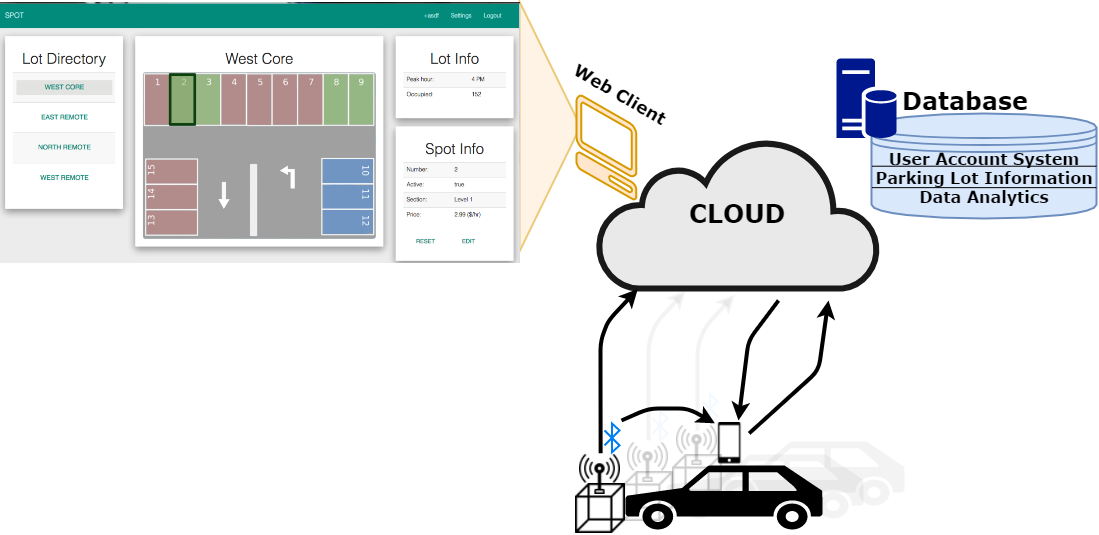
\includegraphics[width=0.85\textwidth]{pictures/SystemOverview.png}
\caption{System overview diagram showing communication paths between the cloud, sensor modules, website, and phone application.}
\end{figure}
%%%%%%%%%%%%%%%%%%%%%
For our implementation, we focus on if a car is about two feet in front, we will capture the license plate, run license plate recognition software, then simultaneously update the database with the current information and broadcast a Bluetooth beacon.
That exact same Bluetooth beacon that is broadcasting the uuid, was assigned by the Cloud.
Consequentially, it is picked up by the user’s phone that prompts a user sign-in/sign-up, payment option and a notification if they arrived at the specific stall. 
The Cloud works on providing the user and owner of the parking location an environment where both users can easily navigate and pursue the necessary actions they require. 
While hosting such services, the Cloud also performs its database duties by holding all information for every imaginable aspect: user account, individual sensor status, time of occupancy, structure/section pricing rates, etc.  
SPOT’s eventual goal is to provide a system that works far more efficiently for both drivers and managers of lots compared to today’s current parking system. 